\chapter{Validierung der Optimierungsergebnisse}
\label{cha:Validierung}
%... Verifikation, Auswertung, Lösungsbewertung, Diskussion der Ergebnisse
%Anwendung auf bestehende Systeme, ohne dass die Hardware 
%negative  Ergebnisse 
%lokales minimum 
Das Ziel der Validierung besteht darin, die in der Simulation berechneten Energieeinsparungen am realen System mithilfe des optimierten Parametervektors nachzuweisen. Der Optimierer wurde gegenwärtig nur an einem einzigen Pfad für den Roboter getestet. Von einer Abbildung der Validierung auf weitere Optimierungsversuche wird abgesehen. Diese sind im Einzelfall zu überprüfen. Der Messaufbau ist identisch zu der Beschreibung im Kapitel \ref{sec:modellvalidierung} Validierung des Roboterdynamik-Modells. 
%
\section{Durchführung}
Roboterprogramme werden auf der KR C5 in der Programmiersprache KRL geschrieben. Ein KRL-Programm ist dabei aus einem source-file (src) und einem data-file (dat)  aufgebaut. Der justierte-energieoptimierte Parametervektor $\bm{q}_v$ wird auf der KR C5 zwischen dem Start- und Zielpunkt der letzten Bewegungsbahn des Programms Kleben-Seitenwand als Via-Punkt \lstinline|ViaJustOptUp| im src-file angelegt. 
\begin{lstlisting}[numbers=none]
	;FOLD PTP ViaJustOptUp Vel=100 % PDAT8 Tool[1] Base[0] ;%{PE}
\end{lstlisting}
Ohne einen expliziten Befehl fährt der Roboter den Via-Punkt millimetergenau an und reduziert seine Geschwindigkeit bei Erreichen des Punkts auf Null. In der Problemstellung der Arbeit wurde eine signifikante Abweichung von der originalen Bewegungsdauer als unzulässig definiert. 
Infolgedessen wird der Implementierte Via-Punkt im src-file um den KRL Überschleifbefehl \lstinline|CONT| erweitert. 
%
\begin{lstlisting}[numbers=none]
	;FOLD PTP ViaJustOptUp CONT Vel=100 % PDAT8 Tool[1] Base[0] ;%{PE}
\end{lstlisting}
%
Zusätzlich muss der Robotersteuerung mitgeteilt werden, in welchem Modus der Via-Punkt zu überschleifen ist und welcher Überschleifradius angewendet werden soll. Dies erfolgt im dat-file über die Parameterdefinition \lstinline|PDAT|, welche dem Via-Punkt src-file zugewiesen ist. 
Die Approximationsmethode \lstinline|APO_MODE| wird mit \lstinline|CDIS| festgelegt. Das bedeutet ein Überschleifen beginnt frühestens, wenn die Entfernung zum Punkt den Wert von \lstinline|APO_DIST = 500 mm| unterschreitet \cite[S.~578]{KSS.2023}.
\begin{lstlisting}[numbers=none]
	DECL PDAT PPDAT8={VEL 100.0000,ACC 100.000,APO_DIST 500.000,APO_MODE #CDIS,GEAR_JERK 100.000,EXAX_IGN 0}
\end{lstlisting}
Die maximale Überschleifdistanz wird auf 500 mm festgelegt. Von der Nutzung des maximal möglichen Überschleifradius 1000 mm wird Abstand genommen, um das Risiko einer Kollision des Roboters mit peripheren Bauteilen zu begrenzen. Die neu programmierte Bewegung wird zunächst auf Kollisionsfreiheit durch manuelles Abfahren mit reduzierter Geschwindigkeit in der KUKA Betriebsart T1 getestet. Nach einer Verifizierung der Überschleifbewegung für eine programmierte Geschwindigkeit von 50~\% in der Betriebsart T2 erfolgt die Signalaufzeichnung der justierten-energieoptimierten Trajektorie mit einer programmierten Geschwindigkeit von 100~\%. 
%
\section{Auswertung}
Die über alle sechs Gelenke summierte Leistungsaufnahme des Roboters wird in \ref{fig:pup} abgebildet. 

\begin{figure}[tbph]
	\centering
	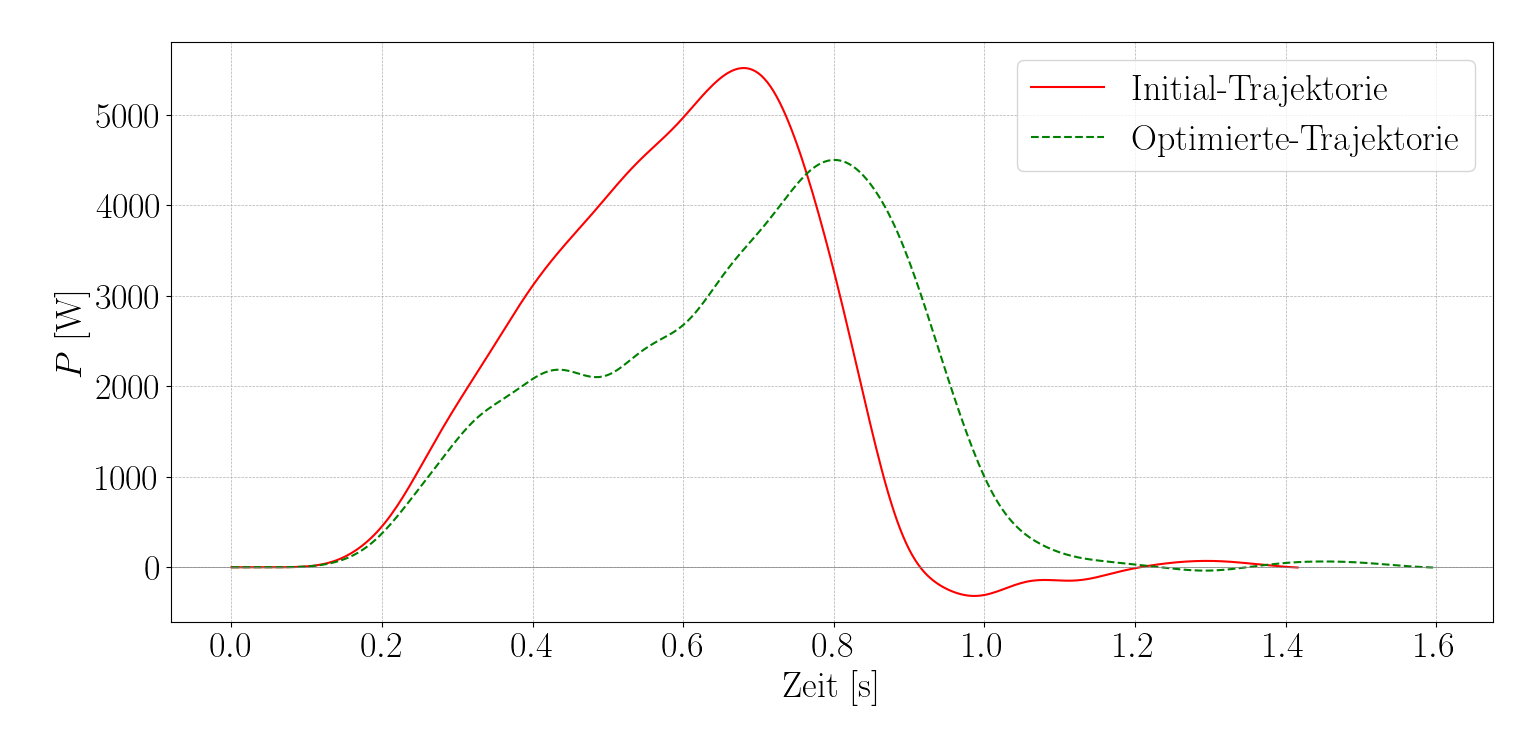
\includegraphics[width=1\linewidth]{images/P_up}
	\caption{Vergleich der summierten Leistungsaufnahme für die initiale Bewegungsbahn und die justierte energieoptimierte, Bewegungsbahn vom letzten Prozesspunkt auf die  Home Position im Programm Kleben-Seitenwand}
	\label{fig:pup}
\end{figure}

Dabei ist eine Zunahme der Bewegungsdauer für die justierte-energieoptimierte Trajektorie um ca. 0,2 s gegenüber der Initial-Trajektorie festzustellen. Die exakte Dauer kann nur näherungsweise angegeben werden. Dies liegt an der im Rahmen der Arbeit entwickelten Datenverarbeitung. Die über den RSI aufgezeichneten und am Server empfangenen Signale werden nachträglich separiert und der einzelnen Bewegungen zugewiesen. Eine neue Bewegung wird beim Durchlaufen einer niedrig gewählten Leistungsschwelle indiziert. Die leichte Zunahme der Bewegungsdauer wird  dem zusätzlichen Programmschritt durch die Definition des Via-Punkts mit \lstinline|CDIS = 500 mm| angerechnet. In der PTP-Bewegungsart führt der Roboter den TCP entlang der schnellsten Bahn zum Zielpunkt \cite[S.~429]{KSS.2023}. Der Via-Punkt hat zur Folge, dass der TCP nicht mehr auf der schnellsten Bahn geführt wird. Die maximal aufgenommene Momentanleistung konnte um ca. 1 kW gesenkt werden. 
Gegenüber der stetig ansteigenden Leistungsaufnahme der Initial-Trajektorie weißt die Leistungskurve der Optimierten-Trajektorie einen Sattel auf.  Der Verlauf der simulierten Leistung, siehe Abbildung \ref{fig:poptfinal}, sowie die im Anhang hinterlegten simulierten Bewegungsdaten weisen dagegen keine Unstetigkeit auf. Die dem Sattel zugrunde liegende temporäre Reduktion der Geschwindigkeit setzt auf der Hälfte der Bewegungsdauer zwischen dem Start und dem Via-Punkt ein. Die Ursache dafür liegt in der Begrenzung der Geschwindigkeit des sechsten Gelenks. In der Konsequenz ist der Optimierer um die Geschwindigkeitsnebenbedienung \ref{eqn:conacc}, sowie die im Kapitel \ref{sec:Nebenbedingungen} genannten und in \cite[S.~5]{Hansen.2012} beschriebenen Formulierungen zur Begrenzung der maximalen Beschleunigung bzw. des maximalen Drehmoments zu erweitern. 
%\begin{figure}[tbph]
%	\centering
%	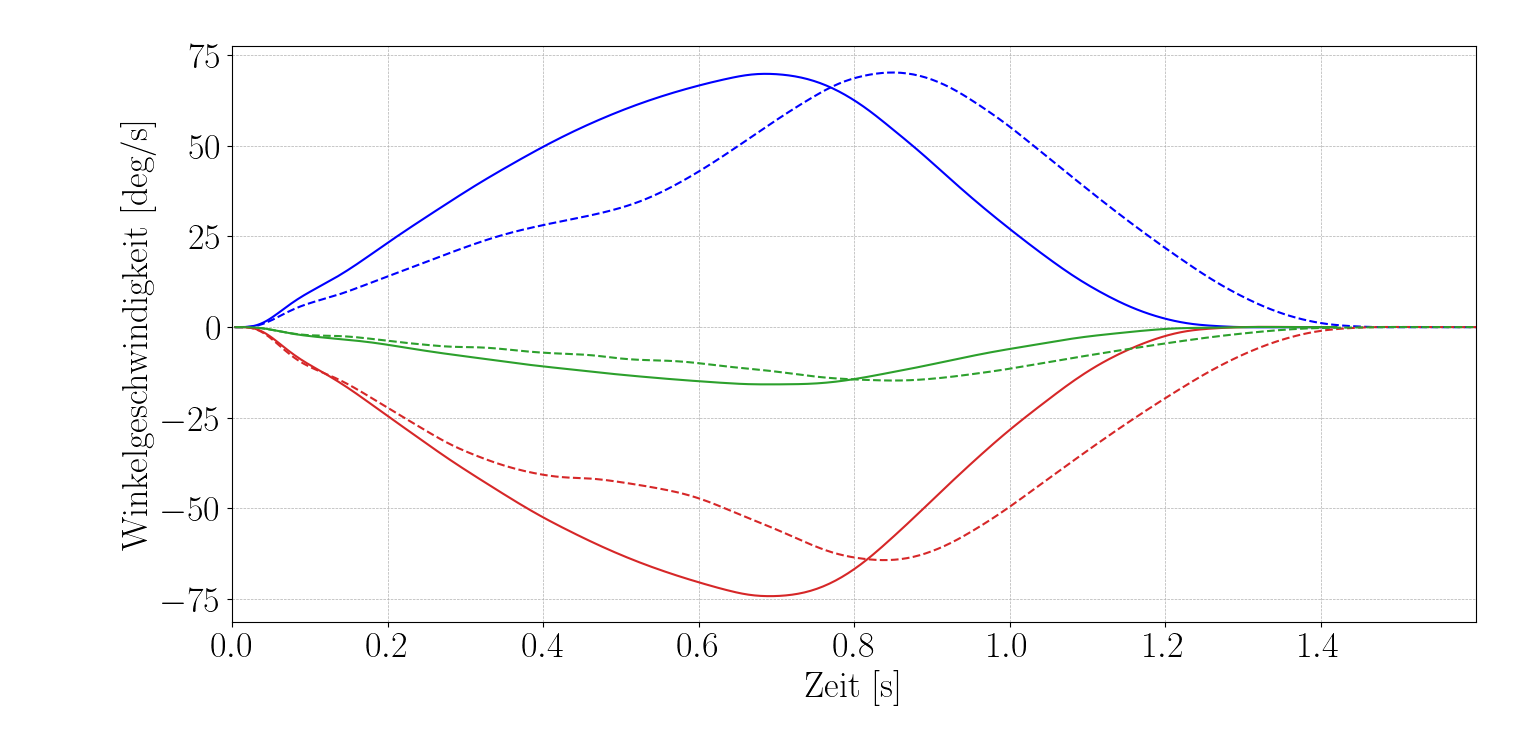
\includegraphics[width=1\linewidth]{images/velposup1}
%	\caption{Winkelgeschwindigkeit in den Gelenken 1-3 Bewegung Zwei}
%	\label{fig:velposup1}
%\end{figure}
Die über den optimierten Via-Punkt erzielte Energieeinsparung wird in der Grafik \ref{fig:eup500} dargestellt. Die Prognose der Simulation, dass die höchste Einsparung für das zweite Gelenk zu verzeichnen ist, wird erfüllt. Wie erwartet ist für den mechanischen Energieverbrauch im ersten Gelenk eine leichte Zunahme festzustellen. Die Optimierungsergebnisse werden in der Konsequenz als plausibel eingestuft. 

\begin{figure}[tbph]
	\centering
	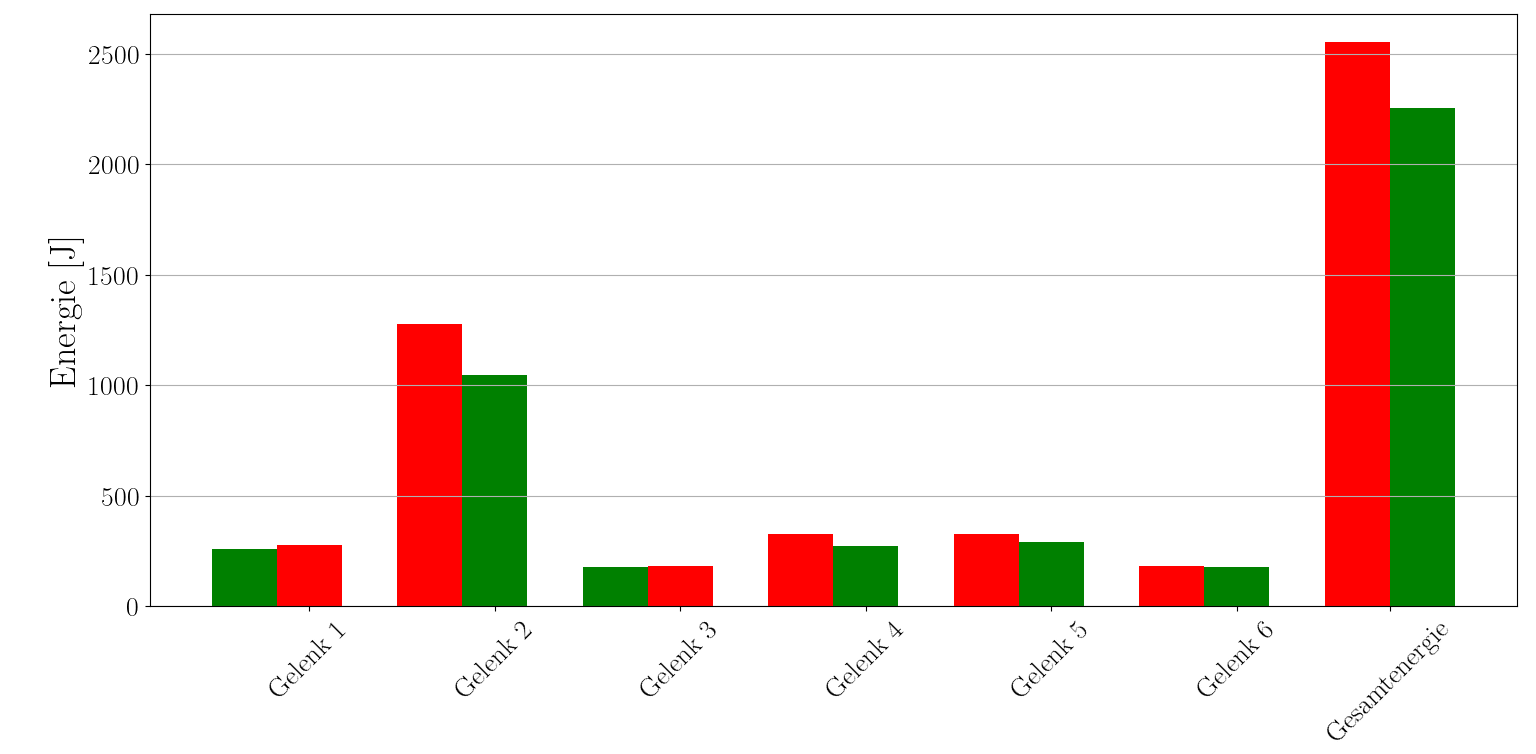
\includegraphics[width=1\linewidth]{images/e_up500}
	\caption{Vergleich des mechanischen Energieverbrauchs für die initiale Bewegungsbahn und die justierte energieoptimierte, Bewegungsbahn vom letzten Prozesspunkt auf die  Home Position im Programm Kleben-Seitenwand}
	\label{fig:eup500}        
\end{figure}